\chapter{Estudo de caso (QIE)}
\label{cap:estudo}
Neste capítulo será descrita a utilização do processo de alinhamento através de um estudo de caso, o QIE. O QIE foi escolhido, pois se trata de um projeto que pretende cruzar informações sobre a comunidade brasileira de Informática na Educação. Este capítulo está estruturado em três seções. A seção \ref{sec:estudo_descricao} apresenta uma descrição do estudo de caso e a conversão dos dados para RDF. A seção \ref{sec:exec_processo} apresenta o passo a passo de como o processo foi executado no estudo de caso. Por fim, a seção \ref{sec:resultados} apresenta os resultados apresentados a partir do alinhamento.

\section{Descrição do estudo}
\label{sec:estudo_descricao}
Para validar a eficácia da solução, foi solicitado a membros da Comissão Especial de Informática na Educação que sugerissem perguntas de interesse sobre a comunidade brasileira de Informática na Educação. Como resultado foi levantado um conjunto contendo mais de 30 questões. A Tabela \ref{tab:questions} apresenta as questões propostas pelos membros.

\begin{table}[!ht]
	\centering
	\caption{Perguntas sugeridas pela comunidade}
	\label{tab:questions}
	\begin{tabular}{|l|l|}
		\hline
		\textbf{ID}  & \textbf{Questões}                                                                          \\ \hline
		Q01 & Quantos pesquisadores de Informática na Educação (IE) há na comunidade?                                                            \\ \hline
		Q02 & Quais são os pesquisadores em IE no Brasil?                                                              \\ \hline
		Q03 & Onde estão os pesquisadores de IE no Brasil? (Estado)                                                              \\ \hline
		Q04 & Onde estão trabalhando os pesquisadores de IE no Brasil? (Universidade)                                                        \\ \hline
		Q05 & Quais pesquisadores de IE no Brasil são doutores?                                                               \\ \hline
		Q06 & Quantos pesquisadores de IE no Brasil são doutores?                                                             \\ \hline
		Q07 & Quem dos pesquisadores de IE no Brasil possui marca registrada?                                                                \\ \hline
		Q08 & Onde os pesquisadores de IE no Brasil fizeram o Doutorado?                                                \\ \hline
		Q09 & Onde os pesquisadores de IE no Brasil fizeram os pós-doutorados?                                            \\ \hline
		Q10 & Quantas publicações o autor “z” tem no evento “x” (SBIE/WIE) da área de IE?                                \\ \hline
		Q11 & Quantos trabalhos foram publicados no evento “x” (SBIE/WIE) da área de IE?                                 \\ \hline
		Q12 & Quantos autores publicaram no evento “x” (SBIE/WIE) da área de IE?                                         \\ \hline
		Q13 & Quantos artigos foram publicados no periódico “y” (RBIE) da área de IE?                                \\ \hline
		Q14 & Lista de doutores que publicaram na RBIE e seus e-mails.                                                  \\ \hline
		Q15 & Lista de autores da comunidade de IE no Brasil, com competência e e-mail.                                            \\ \hline
		Q16 & Lista de artigos publicados na RBIE - Geral.                                       \\ \hline
		Q17 & Quantos pesquisadores da comunidade de IE são bolsistas PQ/DT e qual o nível?                           \\ \hline
		Q18 & Quais são as principais competências da comunidade de IE?                         \\ \hline
		Q19 & Quais conceitos são explorados pelos pesquisadores de IE no Brasil?                                                   \\ \hline
		Q20 & Quais os temas são mais pesquisados em IE no Brasil?                                        \\ \hline
		Q21 & Quais pesquisadores de IE no Brasil colaboram entre si?                                           \\ \hline
		Q22 & Quais instituições que os pesquisadores de IE no Brasil atuam que colaboram entre si?                                            \\ \hline
		Q23 & Quais são os trabalhos relacionados publicados no SBIE, WIE e RBIE?                                              \\ \hline
		Q24 & Como os conceitos explorados nas publicações de IE evoluem ao longo do tempo?                   \\ \hline
		Q25 & Mapa de tendências de pesquisa em IE no Brasil em uma linha do tempo.                             \\ \hline
		Q26 & O quão um pesquisador X está publicando no SBIE, WIE e RBIE ao longo do tempo?    \\ \hline
		Q27 & Lista de bolsistas de produtividade de pesquisadores em IE no Brasil.                                               \\ \hline
		Q28 & Quais as instituições que os pesquisadores de IE no Brasil atuam?                                                            \\ \hline
% * <profsean@gmail.com> 2017-01-19T00:58:04.703Z:
% 
% > Quais as instituições que os pesquisadores de IE no Brasil atuam?
% Tem que verificar a diferença desta com a  Q04...
% 
% ^ <armandobs14@gmail.com> 2017-01-20T04:51:29.061Z:
%
% A diferença entre as duas questões é que uma está voltada para a cidade e outra para as instituições.
%
% ^ <armandobs14@gmail.com> 2017-01-20T04:51:31.469Z.
		Q29 & Quais autores da comunidade de IE no Brasil publicaram na conferência "X"?                                      \\ \hline
		Q30 & Quantos pesquisadores de IE no Brasil estão em Programas de Pós-Graduação de Computação?      \\ \hline
		Q31 & Quem são os maiores especialistas em recursos digitais e objetos de aprendizagem no Brasil? \\ \hline
	\end{tabular}
\end{table}

De acordo com as perguntas realizadas, pode-se perceber que para responder algumas delas é necessário o cruzamento de diferentes fontes de informações dos pesquisadores e suas publicações, sendo elas a Revista Brasileira de Informática na Educação\footnote{\url{http://www.br-ie.org/pub/index.php/rbie}} (RBIE), Workshop de Informática na Escola\footnote{\url{http://www.br-ie.org/pub/index.php/wie }} (WIE), Simpósio Brasileiro de Informática na Educação\footnote{\url{http://www.br-ie.org/pub/index.php/sbie}} (SBIE) e curriculum Lattes\footnote{\url{http://lattes.cnpq.br}}. Vale a pena ressaltar que os \textit{datasets} foram disponibilizados como arquivos XML, sendo necessário transformá-los para RDF.

Para modelar os dados, foram utilizadas as ontologias dac\footnote{\url{https://github.com/josmarios/dac/blob/master/Ontologies/dacV2.1.owl}} e lattes\footnote{\url{https://github.com/armandobs14/lattes/blob/master/lattes.owl}}. A primeira tem o objetivo de modelar o domínio de publicação (ver Figura \ref{fig:dac}). A segunda foi construída para modelar o domínio do lattes (ver Figura \ref{fig:lattes}).

\begin{figure}[!ht]
	\centering
	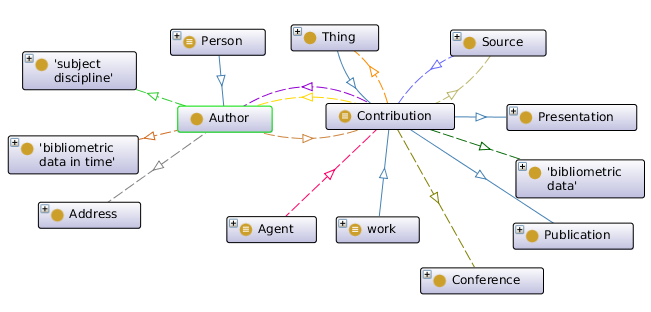
\includegraphics[width=0.9\textwidth]{./imagens/dac-mainview.png}
	\caption{Taxonomia da ontologia dac}
	\label{fig:dac}
\end{figure}

\begin{figure}[!ht]
	\centering
	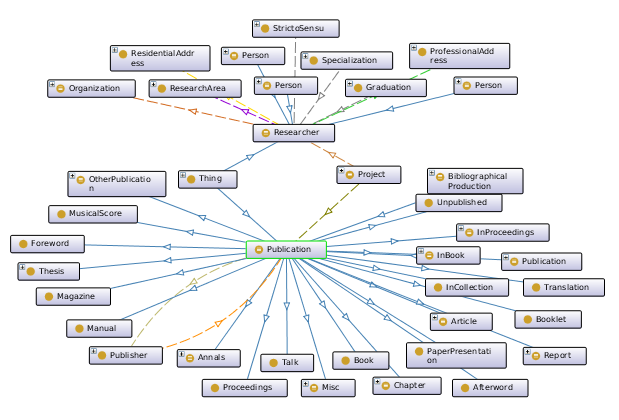
\includegraphics[width=0.9\textwidth]{./imagens/lattes-mainview.png}
	\caption{Taxonomia da ontologia lattes}
	\label{fig:lattes}
\end{figure}

Para transformar os dados para RDF foi utilizada a ferramenta OpenRefine\footnote{\url{http://openrefine.org}} com a extensão para suportar RDF. Essa ferramenta foi selecionada devido a sua facilidade para criar os \textit{templates} de transformação. Após a transformação dos dados, as ontologias e os dados foram persistidos no Virtuoso\footnote{\url{https://virtuoso.openlinksw.com}}. A Figura \ref{fig:conversao} representa o processo de conversão dos dados.

\begin{figure}[!ht]
	\centering
	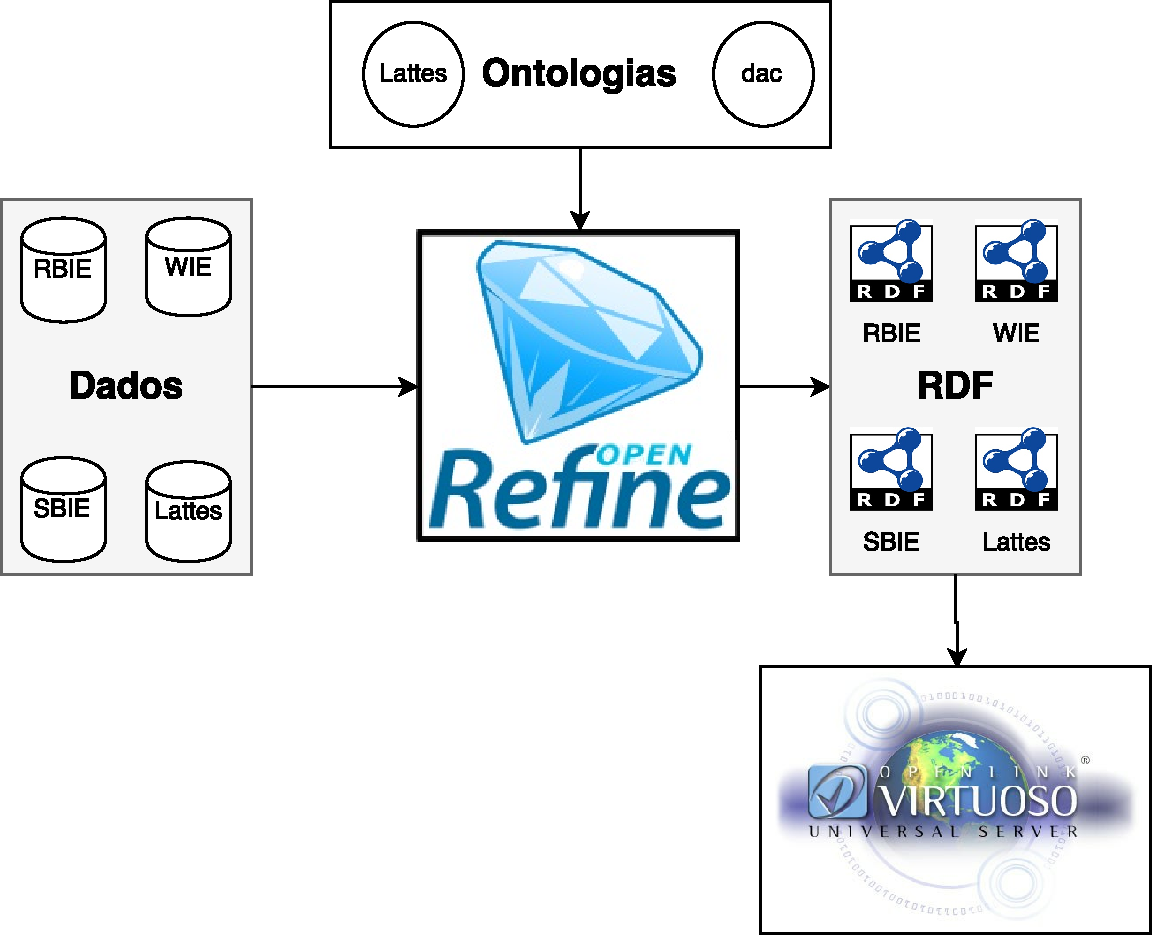
\includegraphics[width=0.8\textwidth]{./imagens/conversao.pdf}
	\caption{Processo de conversão para rdf}
	\label{fig:conversao}
\end{figure}

Com o processo de conversão dos dados foram geradas 1,1 milhão de triplas, sendo distribuídas da seguinte forma: (96\%, 1.094.307 triplas) pertencem ao Lattes, (1,61\%; 18.363 triplas) pertencem ao SBIE, (1,21\%; 14.601 triplas) pertencem ao WIE e (1,1\%; 12.503 triplas) pertencem ao RBIE.

\newpage
\section{Execução do processo}
\label{sec:exec_processo}
Nesta seção descreve-se como foi realizada cada uma das etapas do processo de correspondência. 

\subsection{Selecionar \textit{Datasets}}
\label{sub:selecionar_datasets}
Esta etapa refere-se à seleção de quais \textit{datasets} são utilizados como entrada para o processo de correspondência de instâncias. Vale ressaltar que dois ou mais \textit{datasets} podem ser selecionados. Neste contexto, foram selecionados os \textit{datasets} do RBIE, SBIE, WIE e Lattes.
  
\subsection{Identificar Conceitos}
Esta etapa do processo expõe a seleção dos conceitos (principal e relacionados), que são utilizados no processo. Atualmente existe apenas uma restrição quanto a seleção dos conceitos, nesta é possível selecionar apenas um conceito principal.

\subsubsection{Conceito Principal}
Como descrito na seção \ref{sec:prop_identificar}, para facilitar a identificação do conceito principal por parte do usuário, a consulta \ref{lst:sparql} foi desenvolvida. A Tabela \ref{tab:estudo_sparql1} apresenta os resultados obtidos através execução da consulta. 

\begin{table}[h]
	\centering
	\caption{Conceito da ontologia e quantidade de instâncias}
	\label{tab:estudo_sparql1}
	\begin{tabular}{@{}|l|r|@{}}
		\hline
		\multicolumn{1}{|c|}{\textbf{Conceitos}}               & \multicolumn{1}{c|}{\textbf{quantidade}} \\ \hline
		http://www.ic.ufal.br/dac/Contribution               & 868752                              \\ \hline
		http://www.ic.ufal.br/dac/Author                     & 155680                              \\ \hline
		http://www.ic.ufal.br/lattes/DoctoralDegree          & 2387                                \\ \hline
		http://www.ic.ufal.br/lattes/Graduation              & 2195                                \\ \hline
		http://www.w3.org/2002/07/owl\#Class                 & 1680                                \\ \hline
		http://www.ic.ufal.br/lattes/Course                  & 1186                                \\ \hline
		http://www.w3.org/1999/02/22-rdf-syntax-ns\#List     & 204                                 \\ \hline
		http://www.w3.org/2002/07/owl\#Restriction           & 161                                 \\ \hline
		http://www.w3.org/2002/07/owl\#ObjectProperty        & 128                                 \\ \hline
		http://www.w3.org/2000/01/rdf-schema\#Class          & 60                                  \\ \hline
		http://www.w3.org/2002/07/owl\#Ontology              & 24                                  \\ \hline
		http://www.w3.org/1999/02/22-rdf-syntax-ns\#Property & 23                                  \\ \hline
		http://purl.org/dc/terms/AgentClass                  & 3                                   \\ \hline
	\end{tabular}
\end{table}

O conceito \textbf{\textit{Author}}, que representa a segunda maior quantidade de instâncias nos dados, foi selecionado como conceito principal. A escolha desse conceito deu-se não pela quantidade de instâncias, mas por questões estratégicas, visto que a proposta deste estudo de caso é cruzar informações de pesquisadores.

\subsubsection{Conceito Relacionado}
Para selecionar o conceito relacionado que será utilizado, foi executada a consulta \ref{lst:sparql2}. A Tabela \ref{tab:estudo_sparql2} apresenta os conceitos relacionados ao conceito principal previamente selecionado.

\begin{table}[h]
	\centering
	\caption{Lista com conceitos relacionados}
	\label{tab:estudo_sparql2}
	\begin{tabular}{@{}|l|@{}}
		\hline
		\multicolumn{1}{|c|}{\textbf{Conceito Relacionado}}        \\ \hline
		http://www.ic.ufal.br/dac/Contribution                     \\ \hline
		http://www.ic.ufal.br/lattes/Software                      \\ \hline
		http://www.ic.ufal.br/lattes/TradeMark                     \\ \hline
		http://xmlns.com/foaf/0.1/Organization                     \\ \hline
		http://www.ic.ufal.br/lattes/Organization                  \\ \hline
		http://www.nees.com.br/boa-moradia/crawler/LocalityAddress \\ \hline
		http://www.ic.ufal.br/lattes/DoctoralDegree                \\ \hline
		http://www.ic.ufal.br/lattes/Graduation                    \\ \hline
		http://www.ic.ufal.br/lattes/MastersDegree                 \\ \hline
	\end{tabular}
\end{table}
 
O conceito \textbf{\textit{Contribution}} foi selecionado como conceito relacionado. Esse conceito foi utilizado durante o alinhamento em cascata. Vale ressaltar que mais de um conceito relacionado pode ser selecionado.
 
\subsection{Listar Recursos}
A lista de recursos é gerada de forma automática com base nos conceitos selecionados anteriormente. A partir da lista de recursos são montados os pares candidatos. Vale ressaltar que no estudo em questão um \textit{dataset} pode conter mais de uma instância para a mesma entidade do mundo real (e.g. mais de uma URI para o mesmo pesquisador). Dessa forma, foram gerados pares candidatos dentro do mesmo \textit{dataset}, caracterizando o alinhamento interno.

\subsection{Alinhar Dados}
A etapa de alinhamento é responsável por determinar a correspondências entre as instâncias. Neste processo existem duas abordagens de alinhamento sendo elas simples e em cascata. Na abordagem simples, os recursos são comparados diretamente, explorando as propriedades e suas características. Na abordagem em cascata os recursos são comparados a partir dos recursos relacionados.

\subsubsection{Alinhamento Simples}
Assim como outras abordagens para a correspondência de instâncias \cite{zhang2016rimom}, também foram utilizadas funções que analisam a similaridade entre dois recursos. Para determinar a similaridade entre os pares foi utilizada a função \ref{eq:similaridade}. Essa função de similaridade gera valores entre 0 e 1, sendo 0 totalmente distintos e 1 iguais. Além da função utilizada, foram definidos limiares (\textit{threshold}). Isso quer dizer que valores de similaridade acima do limiar eram considerados correspondentes. 

Inicialmente o valor do limiar foi definido de forma arbitrária e posteriormente ajustado com ajuda de testes. Para isso, o mesmo \textit{dataset} era alinhado diversas vezes utilizando um valor de limiar para cada execução. Por fim, o valor do limiar foi estabelecido em 0.88.
% * <profsean@gmail.com> 2017-01-19T01:16:39.223Z:
% 
% > e posteriormente ajustado com ajuda de testes. Nesses testes eram avaliados vários limiares com o objetivo de escolher o de melhor custo/benefício. Por fim, o valor do limiar foi estabelecido em 0.88.
% Isto poderia ser melhor explicado...
% 
% ^ <armandobs14@gmail.com> 2017-01-20T04:59:35.197Z:
%
% Alterei algumas coisas, espero ter esclarecido mais.
%
% ^ <armandobs14@gmail.com> 2017-01-20T04:59:36.652Z.


\subsubsection{Alinhamento em Cascata}
O alinhamento em cascata consiste em alinhar instâncias do recurso principal a partir de recursos relacionados. Esta etapa do processo é executada para cada um dos conceitos relacionados selecionados na etapa de identificação de conceitos e consiste de três atividades:
\begin{itemize}
	\item \textbf{Alinhar recursos relacionados:} O alinhamento simples é executado entre as instâncias que pertencem ao conceito relacionado;
	
	\item \textbf{Recuperar instâncias do conceito principal:} A partir do alinhamento entre instâncias de recurso relacionado, as instâncias que pertencem ao conceito principal são recuperadas.
	
	\item \textbf{Alinhar instâncias do conceito principal:} A partir das instâncias recuperadas novos pares candidatos são gerados e passados como entrada para o alinhamento simples.
\end{itemize}


\section{Resultados}
\label{sec:resultados}
Os resultados apresentados nessa seção estão separados em duas partes. A primeira consiste dos alinhamentos gerados. A segunda aborda as respostas das perguntas realizadas pela comunidade.

\subsection{Alinhamentos}
Após a realização do alinhamento por parte da ferramenta, foi realizado um levantamento, a partir do qual foi possível gerar informações como a quantidade de recursos são repetidos nas bases, total de recursos alinhados com o perfil Lattes, bem como precisão, revocação e medida-f \cite{goutte2005probabilistic} para analisar a confiabilidade dos alinhamentos (ver Tabela \ref{tab:case_study}). Vale ressaltar que o alinhamento de referência foi gerado manualmente com o auxílio de especialistas no domínio.
% * <profsean@gmail.com> 2017-01-19T01:19:01.024Z:
% 
% > para analisar a confiabilidade dos alinhamentos
% Como isto foi feito? Alguém teria que fazer a anotação...
% 
% ^ <armandobs14@gmail.com> 2017-01-20T05:02:01.015Z:
%
% Os alinhamento de referência foi gerado manualmente.
%
% ^ <armandobs14@gmail.com> 2017-01-20T05:02:03.491Z:
%
% Os alinhamento de referência foi gerado manualmente.
%
% ^ <armandobs14@gmail.com> 2017-01-20T05:02:07.468Z.

%\begin{landscape}
\begin{table}[!ht]
	\centering
	\caption{ Resultado dos alinhamentos com relação aos dados do Lattes}
	\label{tab:case_study}
	%\begin{tabular}{|p{1cm}|p{2cm}|p{2cm}|p{1cm}|p{1cm}|p{2cm}|p{2cm}|p{2cm}|}
	\begin{tabular}{|c|c|c|c|}
		\hline
		\textbf{Dataset}	&	\textbf{RBIE}	&	\textbf{SBIE}	&	\textbf{WIE}  \\ \hline
		\textbf{Iniciais}	&	1118	&	1687	&	1952 \\ \hline
		%\textbf{Alinhamentos}	&	276	&	1742	&	1637  \\ \hline
		%\textbf{Recursos Alinhados}	&	1029	&	141	&	1405 \\ \hline
		\textbf{Finais}	&	806	&	1032	&	1098 \\ \hline
		\textbf{Perfis com Lattes*}	&	92.03\% (1029)	&	71.54\% (1207)	&	75.20\% (1468) \\ \hline
		\textbf{Perfis com Lattes**}	&	89.06\% (717)	&	70.16\% (792)	&	67.48\% (741) \\ \hline
		\textbf{P | R | F}	&	0.97 | 1 | 0.98	&	0.94 | 1 | 0.97 	&	0.84 | 1 | 0.91 \\ \hline
	\end{tabular}
\end{table}
* - com repetição
** - sem repetição
%\end{landscape}

\subsection{Respostas}
O processo de correspondência de instância permite não só identificar as instâncias que se referem a mesma entidade, mas também permite que informações complementares sejam integradas. Dessa forma, foi necessário consultar mais de uma base ao mesmo tempo para responder às perguntas feitas pela comunidade. Devido à quantidade de perguntas feitas, apenas algumas delas serão apresentadas a seguir.

Outro fator que deve ser ressaltado trata-se de problemas nos dados que eram fornecidos pelos autores (quantidade de autores diferentes para o mesmo artigo, formatação do nome). Além disso, foi possível notar também o fornecimento de informação inverídica, onde 77 autores usaram o mesmo e-mail (autor@email.com).

\subsubsection{Q03 - Onde estão os pesquisadores de IE no Brasil? (Estado)}
Através desta pergunta é possível saber onde os pesquisadores que publicaram no RBIE, SBIE ou WIE trabalham. Essa informação é obtida através do endereço profissional que pode ser encontrado no perfil do curriculum Lattes de cada pesquisador. Desta forma, para responder a esta pergunta, é necessário identificar o perfil desses pesquisadores no curriculum Lattes.

A consulta \ref{lst:where} recupera o endereço profissional dos pesquisadores que publicaram no WIE. Na linha 9, a transitividade da propriedade \textit{owl:sameAs} é utilizada com o objetivo de recuperar todos os perfis correspondentes. Para que a consulta não entrasse em loop, foi estabelecido a consulta de até 5 elementos compondo a transitividade. A quantidade de 5 elementos foi escolhida de forma manual, com esse valor foi possível alcançar todas as propriedades possíveis através da transividade.
% * <profsean@gmail.com> 2017-01-19T01:25:56.562Z:
% 
% > Para que a consulta não entrasse em loop, foi estabelecido a consulta de até 5 elementos.
% Por que 5?
% 
% ^ <armandobs14@gmail.com> 2017-01-20T05:10:15.441Z:
%
% O valor de 5 foi escolhido de forma prática. Com esse valor foi possível alcançar todas as propriedades possíveis através da transividade.
%
% ^ <armandobs14@gmail.com> 2017-01-20T05:10:52.237Z.

\begin{lstlisting}[captionpos=b, caption= Consulta para recuperar a concentração de pesquisadores por UF, label=lst:where,
basicstyle=\ttfamily,frame=single]
PREFIX dac:<http://www.ic.ufal.br/dac/>
PREFIX lattes:<http://www.ic.ufal.br/lattes/>
SELECT  ?uf count (distinct ?o) as ?total
FROM <http://www.ic.ufal.br/dac/wie/>
FROM <http://www.ic.ufal.br/dac/author/wie/lattes/alignments/>
FROM <http://www.ic.ufal.br/dac/author/wie/wie/alignments/>
FROM <http://www.ic.ufal.br/dac/lattes/>
WHERE {
?s a dac:Author; owl:sameAs{,5} ?o.
filter regex(?s,"http://www.ic.ufal.br/dac/author/wie/(\\d)+$","i")
filter regex(?o,"http://www.ic.ufal.br/dac/author/lattes/(.)+$","i")
filter not exists {graph<http://www.ic.ufal.br/dac/author/wie/wie/alignments/>{?k owl:sameAs ?s}}
?o lattes:hasProfessionalAddress ?address.
?address lattes:uf ?uf
filter exists {?elem owl:sameAs ?g}
}
group by ?uf
order by desc(?total)

\end{lstlisting}

A Figura \ref{fig:where} apresenta a concentração de pesquisadores por unidade federativa (UF). Este mapa também conta com uma versão iterativa\footnote{\url{https://fiddle.jshell.net/4hernfu6/3/show/}}.

\begin{figure}[!ht]
	\centering
	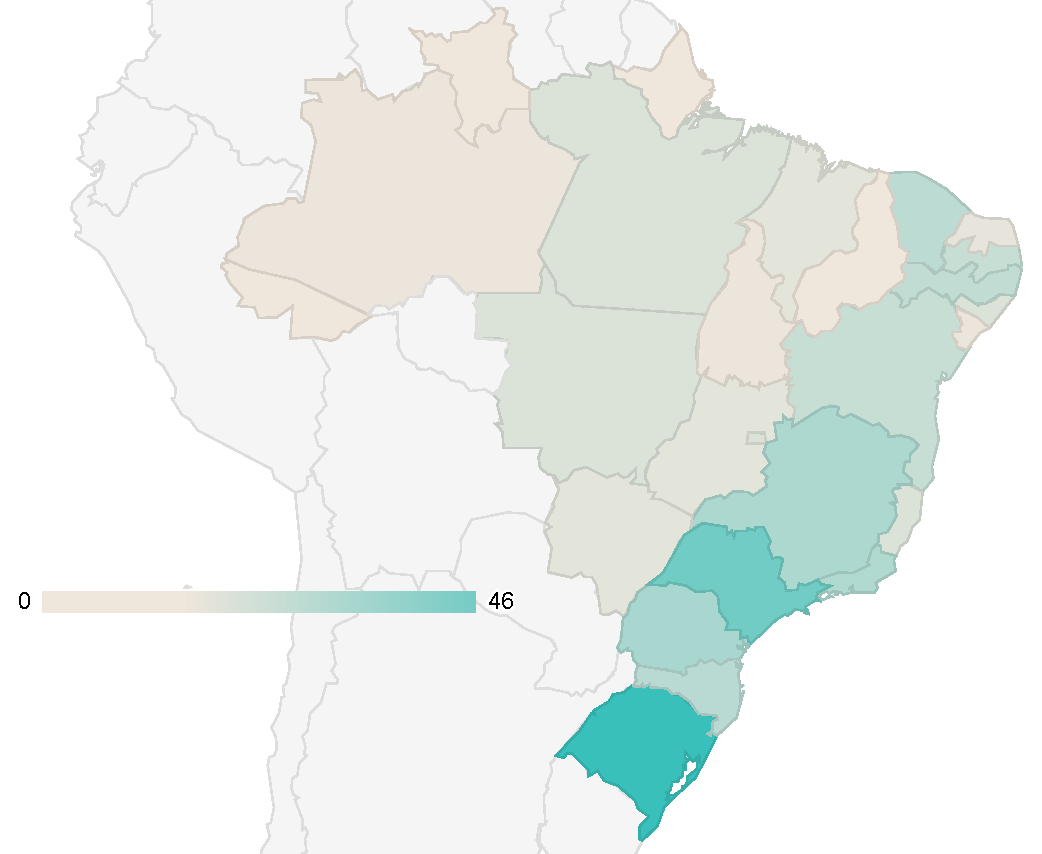
\includegraphics[width=0.8\textwidth]{./imagens/where.pdf}
	\caption{Concentração de pesquisadores por UF}
	\label{fig:where}
\end{figure}

\subsubsection{Q08 - Onde os pesquisadores de IE no Brasil fizeram o Doutorado?}
Através desta pergunta é possível saber onde os pesquisadores que publicaram no RBIE, SBIE e WIE concluíram seus doutorados. Assim como a informação de endereço profissional, esta informação também pode ser obtida através do cruzamento entre essas bases e o Lattes. A consulta \ref{lst:phd} recupera a instituição onde os pesquisadores que publicaram no WIE concluíram seus doutorados.

\begin{lstlisting}[captionpos=b, caption= Consulta para recuperar a concentração de doutorados por universidade, label=lst:phd,
basicstyle=\ttfamily,frame=single]

PREFIX dac:<http://www.ic.ufal.br/dac/>
PREFIX lattes:<http://www.ic.ufal.br/lattes/>

Select ?nameInstitution count( distinct ?g) as ?Count
FROM <http://www.ic.ufal.br/dac/wie/>
from <http://www.ic.ufal.br/dac/author/wie/lattes/alignments/>
from <http://www.ic.ufal.br/dac/author/wie/wie/alignments/>
FROM <http://www.ic.ufal.br/dac/lattes/>

where {
?s a dac:Author; owl:sameAs* ?g.
?g foaf:name ?oname.
filter regex(?s,"http://www.ic.ufal.br/dac/author/wie/(\\d)+$","i")
filter regex(?g,"http://www.ic.ufal.br/dac/author/lattes/(.)+$","i")
filter not exists {graph<http://www.ic.ufal.br/dac/author/wie/wie/alignments/>{?k owl:sameAs ?s}}
?g lattes:hasAcademicDegree ?t.
?t a lattes:DoctoralDegree.
?t lattes:hasInstitution ?institution.
?institution foaf:name ?nameInstitution
}
Order by desc(?Count)
\end{lstlisting}

A Figura \ref{fig:phd} apresenta a concentração de doutorados concluídos por universidade.

\begin{figure}[!ht]
	\centering
	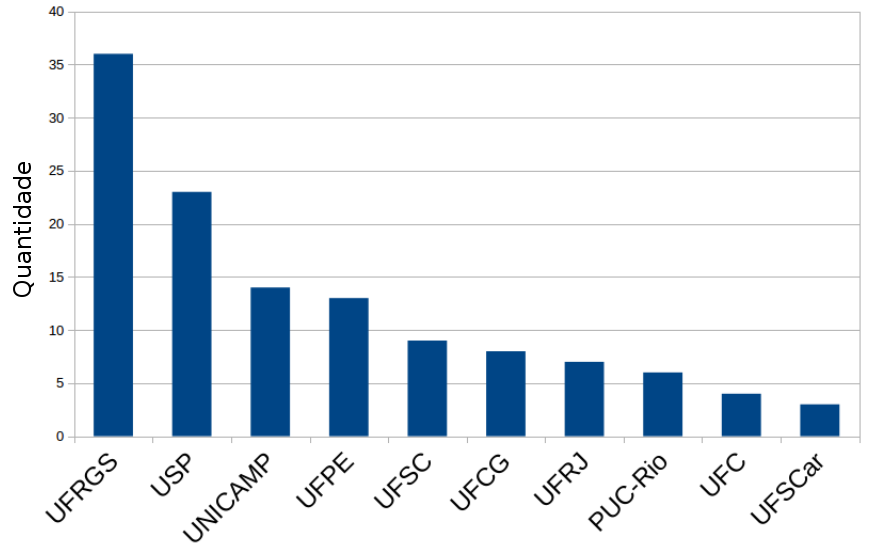
\includegraphics[width=0.8\textwidth]{./imagens/phds.png}
	\caption{Quantidade pesquisadores com doutorado por universidade}
	\label{fig:phd}
\end{figure}